\chapter{Application design}\label{ch:design}

The application is divided into three components:
\begin{itemize}
	\item[\standout{Common}] A library that contains modules that are used
		both by the server and the client. This includes the protocol
		implementation, networking functions, PEM serialization, error
		reporting, console output, \etc; Its code is available in the
		\code{common} folder;
	\item[\standout{Server}] The server application which handles the
		registered users allowing them to log-in and challenge each
		other. Its code is available in the \code{server} folder;
	\item[\standout{Client}] The client application that is used by the user
		to log-in with the server and play the game against other
		players. Its code is available in the \code{client} folder.
\end{itemize}

Each components is divided into a number of modules. Each module provides
functions for a specific functionality of the application and it's compound by a
\emph{C source file} and a \emph{Header file}. All header files are placed under
the \code{include} directory.

\figref{fig:modules} shows all the modules of the developed application along
with their connections with other modules\footnote{Only the main connections are
represented.}.

\begin{figure}[htb]
	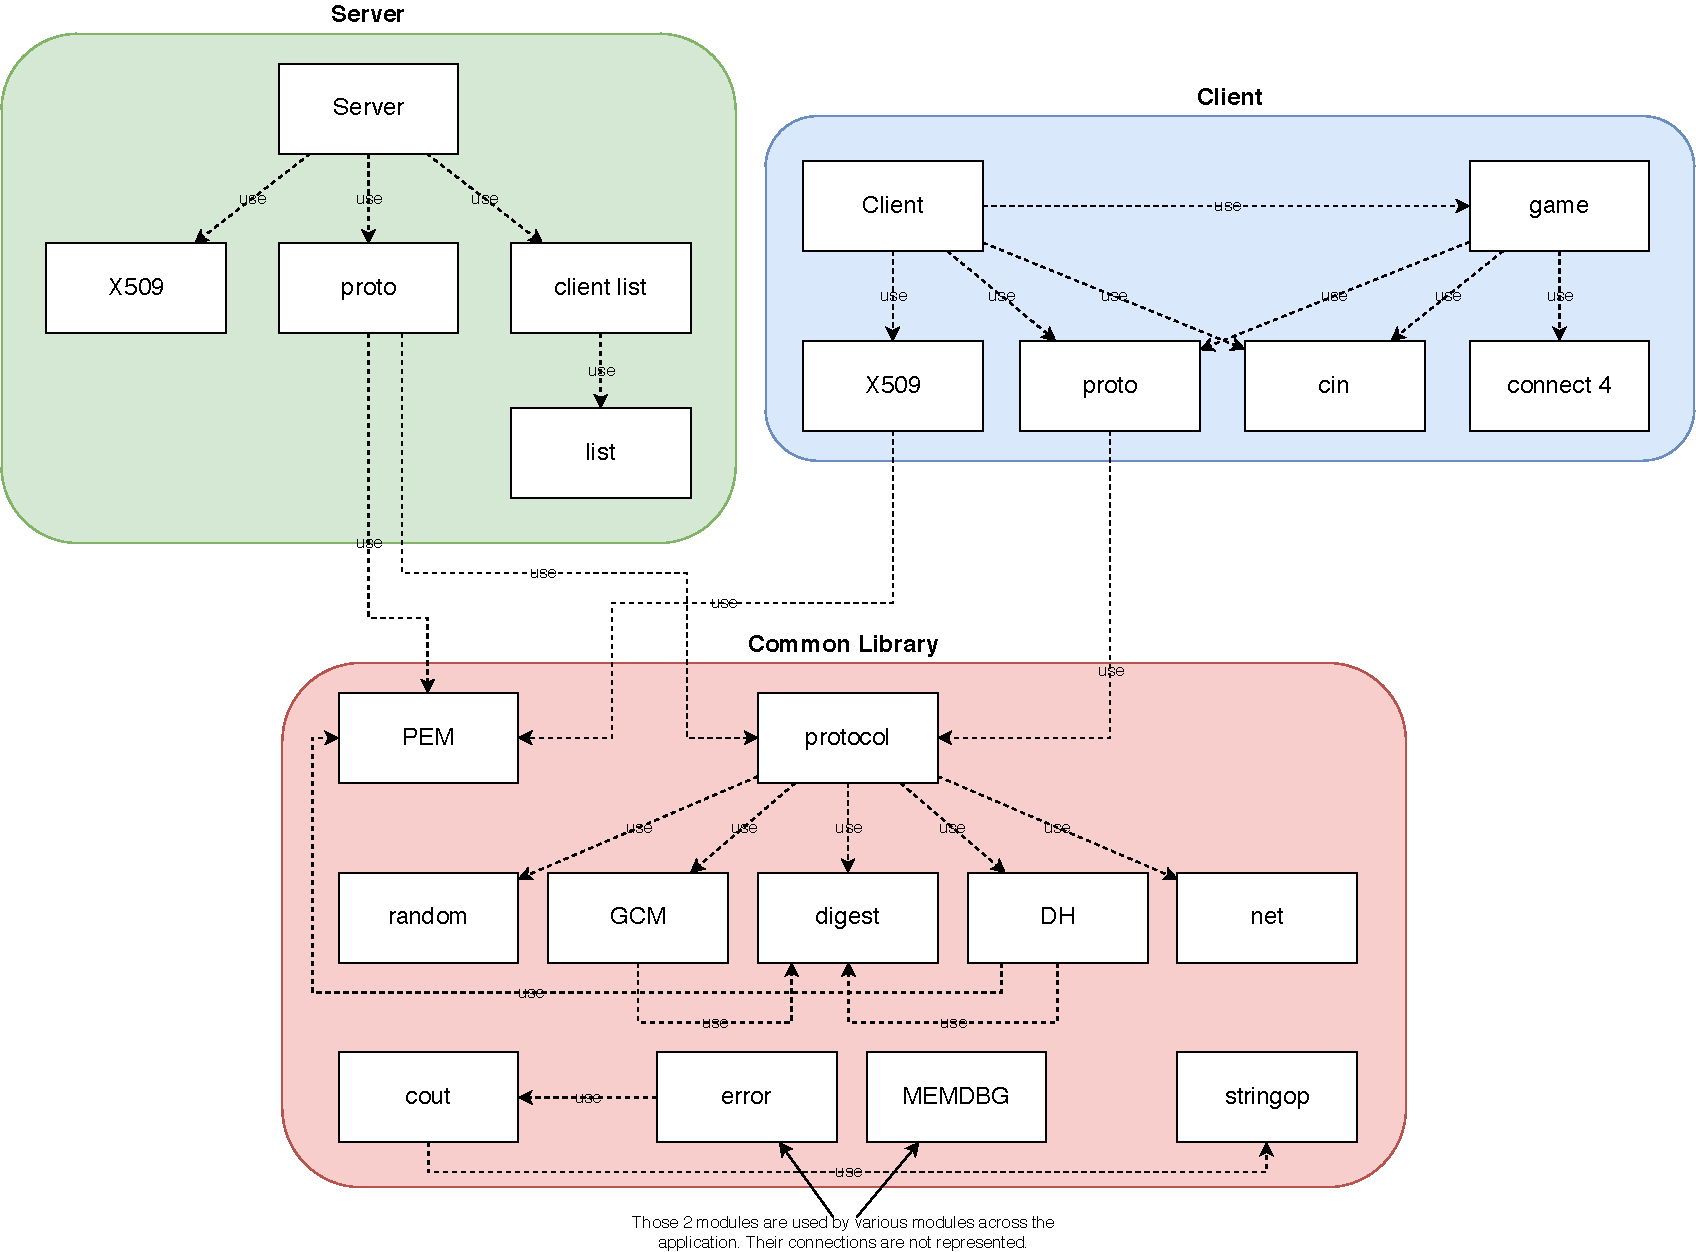
\includegraphics[width=\textwidth]{modules}
	\caption{Application modules}\label{fig:modules}
\end{figure}

\section{Modules description}\label{sec:modules}

This section describe the modules that are part of the application.


\subsection{Common library modules}\label{subsec:commonmod}

This section describes the modules of the common library. For further reference,
the code can be found in the \code{common} folder.

\subsubsection{Protocol}

This module implements the protocol of the application. It contains functions to
send and receive plain, signed or GCM encrypted messages
(\code{proto\_\{send,recv\}\_*}). It also has a function to automatically
determine the format of the message to send (\code{proto\_send}) or receive
(\code{proto\_recv} and \code{proto\_recv\_msg\_type}).

The \code{proto\_verify\_last\_msg} allows to first read a received signed
message and verify the signature afterwards (used by the server when it receives
the first message from the client).

The module also implements the Diffie-Hellman algorithm (using the \code{DH}
module).

This module also defines the \code{PROTO\_CTX} type, that is used to maintain
various informations about the current state of the protocol. Note that this
structure also maintain a pointer to the last received message and the memory
allocated for this message is automatically freed when the application
send/receive the next message (or when the application closes). This saves the
caller the work to free the memory allocated for received messages.

\subsubsection{Networking}

This module contains wrappers for the networking functions \idest{\code{send},
\code{recv}, \code{bind}, \code{accept}, and so on} manly to properly handle
errors.

For when the client initializes a peer-to-peer communication using UDP with
another client, this module also provide a memory buffer to contains all the
data received on the socket until the application reads it. This is useful to
have UDP datagrams to behave like TCP packets (used in the client-server
communication): when an UDP datagram is received, the \code{recvfrom} call
returns the number of bytes requested by the application and immediately
discards any other byte left in the datagram. This contrasts with the behaviour
of the \code{recvfrom} function when it manages TCP packets. So the
\code{recvfrom\_noblock} function wraps around the \code{recvfrom} call in order
to have a behaviour equal to the one we get when using TCP packets.

\subsubsection{Digest}

This module provides functions for hashing any type of data using SHA-256,
signing and verifying messages using RSA\@.

This module also defines the \code{DIGEST\_CTX} type, that is used to maintain
the private RSA key of the user (for signing) and the public key of the peer
(for signature verification).

\subsubsection{Diffie-Hellman (DH)}

This module contains functions used to generate the Diffie-Hellman public key
and to derive a shared secret when the public key of the peer is received.

This module also defines the \code{DH\_CTX} type, that is used to maintain the
generated DH public key and the public key of the peer before the secret
derivation.

\subsubsection{GCM}

This module allows to encrypt and decrypt messages with GCM AES-128. It also
automatically computes a new IV after every message.

This module also defines the \code{GCM\_CTX} type, that is used to maintain the
key and the current IV for the GCM operations, among other data useful to
generate the next IV\@.

\subsubsection{Random}

This module returns a nonce (4 bytes random integer) using the
\code{RAND\_bytes} function from \openssl.

\subsubsection{PEM}

This module provides functions for reading PEM files and
serializing/deserializing PEM data sent over the network.

\subsubsection{Console output (cout)}

This module contains functions to easily print errors on the Standard Error.

\subsubsection{String operations (stringop)}

This module performs string manipulation basic operations: conversion of a
string to another type, lower-casing, trimming, checks (\emph{contains},
\emph{starts}, \emph{ends} conditions).

\subsubsection{Error reporting (error)}

This module provides functions to return an error to the caller of a function
and to print error messages. Every function of the common library that can fail
(and some functions of the client and the server) uses the \code{REPORT\_ERR}
macro to set an error code and an error message. The caller can the inspect the
error code and/or print the error message to the user.

\subsubsection{MEMDBG}

This module is used to check if the application correctly frees the heap after
use: it wraps the \code{alloc} and \code{free} calls and prints a message when
any of these functions are called. It also provides the \code{memdbg\_dump}
macro used to print memory areas on the Standard Output for debugging purposes.

This module is usually disabled. It can be enabled by passing the
\code{-{}-enable-memdbg} option to the \code{configure} script, as explained
in~\appendixref{appendix:howtocompile}.


\subsection{Server modules}\label{subsec:servermod}

This section describes the modules of the server. For further reference, the
code can be found in the \code{server} folder.

\subsubsection{X509}

This module contains just one function that serializes a X509 certificate for
sending it through a socket.

\subsubsection{Proto}

This module builds the messages that must be sent to the clients. It also calls
the functions of the common library's \code{protocol} module to effectively
send/receive the messages.

\subsubsection{Client list}

This module maintain the list of logged-in users in memory. It uses the
\code{list} module to create lists, which is a highly performing list
implementation inspired by the Linux Kernel's \code{klist} implementation.

It builds two lists and an hashtable of lists.

The first list (named \code{unregistered}) contains all the clients that are
connected to the server but have not yet sent their \emph{username} and
\emph{game port} with the initial handshake (they are not ``registered'').

The second list (named \code{client\_list}) contains all the clients that have
completed the initial handshake. The list is maintained ordered by username:
this allows to easily get the list of users ordered by username when a client
asks for it with a \code{PLAYER\_LIST\_REQ} message.

The hashtable is used to rapidly get the client's informations when a message is
received by the server. The clients' data structures are saved in the list
contained in the element at index: \[socknum \bmod HASHTABLE\_SIZE\] where
\(socknum\) is the socket's descriptor number.

\subsubsection{Main module (server)}

The main modules handles all the operations related to the communication with
the clients and the main business logic of the server.

It uses the \code{client\_list} module to maintain a list of all the connected
clients.

The \code{select} call is used to wait on multiple sockets (one for each client)
for a new message. When a message is received, it is processed by an handler
function specific for each message type.


\subsection{Client modules}\label{subsec:clientmod}

This section describes the modules of the client. For further reference, the
code can be found in the \code{client} folder.

\subsubsection{X509}

This module allows to deserialize and verify (against the trusted authority's CA
and CRL files) the certificate received by the server.

\subsubsection{Proto}

This module builds the messages that must be sent to the server or the
opponent's client during a game. It also calls the functions of the common
library's \code{protocol} module to effectively send/receive the messages.

\subsubsection{Console input (cin)}

This module contains functions used to correctly read from the Standard Input.

\subsubsection{Main module (client)}

The main module handles all the operations related to the communication with the
server and user commands.

After the connection to the server, the client enters a \emph{REPL}
(Read-Eval-Print-Loop) loop where it waits for a message from the server or a
command from the user (the client listen on the Standard Input and the socket
simultaneously using the \code{select} function).

For each message that is received by the server, there is an ``handler''
function that handles it. The same applies for the commands from the user.

\subsubsection{Connect 4}

It contains function to initialize the board, check if one of the two players
has won the game after each move and print the board. It also tracks which is
the current active player.

\subsubsection{Game}

This module sets up and manages the game between the player and its opponent. At
the beginning of the game, it initialized a secure session with the other party.
Then, it handles the input from the player when he makes a move in the game and
the messages coming from the opponent.

It uses the \code{Connect 4} module to register each move made in the game and
print the board after each move.

